\documentclass[main, 12pt, fleqn]{subfiles}

\begin{document}
\begin{lect} {2019-09-12}
		
	\begin{Proof}
		\[P = [t_0, t + h]\]
		\[d_k : t_0 = t_0^k < t_1^k < ... < t_j^k < ... < t_{nk}^k = t_0 + h\]
		\[\text{rank } d_k = \lambda_k = \max_{0 \leq j \leq n_k - 1} (t^k_{j + 1} - t^k_j)\]
		\[(3) \q \lambda \us{k \to  + \infty}{\ra 0}\]
		\[(4) \q \left\{ \begin{align}
				&\varphi_k(t_0) = x_0\\
				&\varphi_k(t) = \varphi_k(t_j^k) + X(t_j^k, \varphi_k(t_j^k))(t - t^k_j)
		\end{align} \text{ - ломанные Эйлера}\]
		\[t_j^k \leq t \leq t_{j + 1}^k\]
		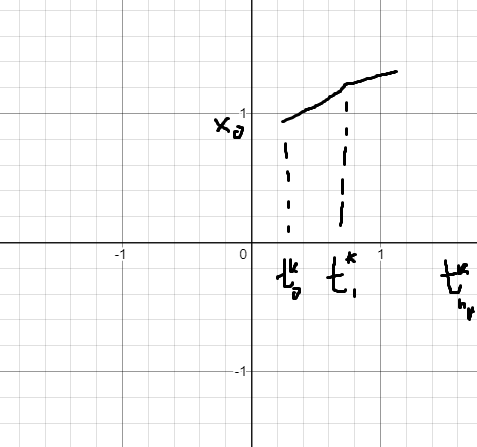
\includegraphics[scale=0.3]{d1.png}
	\end{Proof}
	
	\begin{Lemma} [1]
		\[\text{Определим } \varphi_k (t) \text{ и}\]
		\[|\varphi_k(t) -x_0| \leq M(t - t_0) \q \forall t \in P \q(5)\]
	\end{Lemma}
	
	\begin{Remark}
		\[(5) \Ra t \in P \Ra 0 \leq t - t_0 \leq h \Ra\]
		\[\Ra |\varphi_k(t) - x_0| \leq M \cdot h \leq M \cdot \frac{b}{M} = b \q(6)\]
	\end{Remark}
	
	\begin{Proof} [лемма 1]
		\[\text{Б.И.: } j = 0 \q t \in [t_0^k, t_1^k]\]
		\[\varphi_k(t) = x_0 + X(t_0, x_0) \cdot (t - t_0)\]
		\[\Ra |\varphi_k(t) - x_0| = |\us{\leq M}{X(t_0, x_0)}| (t - t_0) \leq M (t - t_0)\]
		\[\text{И.П.: Пусть } (5) \text{ - выпполняется } \forall t \in [t_0^k, t_j^k]\]
		\[\Ra |\varphi_k (t_j^k) - x_0 | \leq M(t_j^k - t_0) \leq b \Ra (t_j^k, \varphi_k(t_j^k)) \in D\]
		\[t_j^k \leq t < t_{j + 1}^k \]
		\[\text{По (4) имеем: } |\varphi_k(t)| \leq |\varphi_k(t) - x_0| = |\us{\text{инд. предп}}{\varphi_k(t_j^k) - x_0}| + |X(t_j^k, \varphi_k(t_j^k))| (t - t_j^k) \leq\]
		\[\leq M(t_j^k - t_0) + M(t - t_j^k) = M(t - t_0)\]
	\end{Proof}

	\begin{Definition}
		\[(7) \q \left\{ \begin{align}
				&\psi_k(t) = X(t_j^K, \varphi_k(t^k)), \q t_j^k \leq t \leq t^k_{j + 1} \q\q j = 0,..., n_k - 1\\
				&\varphi_k(t^k_{nk}) = X(t_{nk}^k, \varphi_k (t_{nk}^k)) 
		\end{align}\q \]
	\end{Definition}

	\begin{Lemma} [2]
		\[\varphi_k(t) = x_0 + \int_{t_0}^t \psi_k(\tau) d\tau \q\q (8)\]
	\end{Lemma}

	\begin{Proof}
		\[\text{Б.И.: } j = 0 \q t \in [t_0^k, t_1^k]\]
		\[\varphi_k(t) = x_0 + X(t_0, x_0) (t - t_0) = x_0 + \int_{t_0}^t \us{= \psi_k(t)}{X(t_0, x_0)} d\tau\]
		\[\text{Пусть } [t \in [t_0^k, t_j^k] \Ra \varphi_k(t_j^k) = x_0 + \int_{t_0}^{t_j^k} \psi_k (\tau) d \tau \]
		\[\text{И.П.: }t \in [t_j^k, t_{j+1}^k]\]
		\[\Ra \varphi_k(t) = \varphi(t_j^k) + X(t_j^k, \varphi_k(t_j^k)) (t - t_j^k) = \]
		\[= x_0 + \int_{t_0}^{t_j^k} \psi_k(\tau)d\tau + \int_{t_j^k}^{t} X (t_j^k, \varphi_k(t_j^k)) d\tau = x_0 + \int_{t_0}^t \psi_k (\tau) d\tau\]
	\end{Proof}

	\begin{Lemma} [3]
		\[\{\varphi_k(t)\}_{k = 1}^\infty \text{ - равномерно огр., равностепенно непр. для } t \in P\]
	\end{Lemma}

	\begin{Proof}
		\[\text{По пункту (6) } |\varphi_k(t)| \leq |\varphi_k(t) - x_0| + |x_0| \leq b + |x_0| \q \forall k \in \N\]
		\[\mathcal{E} > 0 \q \delta \]
		\[|\ol{t}- \ol{\ol{t}}| < \delta \q (\ol{t}, \ol{\ol{t}} \in P)\]
		\[|\varphi_k(\ol{t}) - \varphi_k(\overline{\overline{t}})| = 
		|\int_{\overline{\overline{t}}}^{\overline{t}} \psi_k(\tau)d\tau | \leq 
	|\int_{\overline{\overline{t}}}^{\overline{t}} |\psi_k(t)| d\tau  | \leq\]
		\[\leq M\delta = \mathcal{E}\]
	\end{Proof}

	\[\exists \text{ подпослед. } \{\varphi_k(t)\}^\infty_1 \q t \in P\]
	\[(9) \q \varphi_{k}(t) \os{P}{\us{k \to +\infty}{\rightrightarrows}} \varphi(t) \text{ (тут должны быть $k_m$, но мы их не будем писать)}\]
	\[\varphi(t) \text{ - непр и } |\varphi(t) - x_0| \leq b\]
	
	\begin{Lemma} [4]
		\[(10) \q\psi_k(t) \os{P}{\us{k \to +\infty}{\rightrightarrows}} X(t, \varphi(t))\]	
	\end{Lemma}
	
	\begin{Proof} [лемма 4]
		\[X(t, x) \in C(D) \Ra X(t, x) \text{ - равном непр. на }D\]
		\[\Ra \forall \mathcal{E} > 0 \exists \delta > 0 : \forall (\overline{t}, \overline{x}), 
		(\overline{\overline{t}}, \overline{\overline{x}}) \in D\]
		\[|\overline{t} - \overline{\overline{t}}| < \delta, \q |\overline{x} - \overline{\overline{x}}| < \delta \Ra\]
		\[\Ra |X(\overline{t}, \overline{x}) - X(\overline{\overline{t}}, \overline{\overline{x}})| 
		< \frac{\mathcal{E}}{2}\]
		\[\text{фикс } \mathcal{E} > 0 \Ra \exists \delta > 0\]
		\[(12) \q|X(t, \varphi(t)) - \psi_k(t) | \leq \us{(1)}{|X(t, \varphi(t)) - X(t, \varphi_k(t))|} + 
		\us{(2)}{|X(t, \varphi_k(t) - \varphi_k(t)|}\]
		\[\text{из } (9) \q \Ra \exists k_1 : \forall k > k_1 \q |\varphi_k(t) - \varphi(t)| < \delta \q \forall t \in P\]
		\[\Ra \underbrace{|...|}_{(1)} < \frac{\mathcal{E}}{2} \]
		\[t = t_{nk}^k \Ra \underbrace{|...|}_{(2)} = 0 \text{ по (7)} \]
		\[ \text{Если } [t \neq t_{nk}^k \ra \exists j \in \{0, 1, ..., n_k - 1\} : t \in [t_j^k, t_{j + 1}^k ) \]
		\[\text{И тогда } \underbrace{|...|}_2 = |X(t, \varphi_k(t)) - X(t_j^k, \varphi_k(t_j^k))|\]
		\[\exists k_2 : \forall k > k_2 \q \lambda_k < \min(\delta, \frac{\delta}{M}) \q (\text{из } (3))\]
		\[\Ra (t - t_j^k) < (t_{j + 1}^k - t_j^k ) \leq \lambda_k < \delta\]
		\[|\varphi_k(t) - \varphi_k(t_j^k)| \leq |\int_{t_j^k}^t |\us{\leq M}{\psi_k(t)}| \leq 
		M(\us{\leq \lambda_k}{t - t^k_j}) < M \frac{\delta}{M} = \delta\]
		\[\Ra |\underbrace{...}_{(2)} | < \frac{\mathcal{E}}{2} \text{ по (11)}\]
		\[\Ra \forall k > \max(K_1, k_2) \q\q |X(t, \varphi(t)) - \psi_k(t)| < \frac{\mathcal{E}}{2} + 
		\frac{\mathcal{E}}{2} = \mathcal{E} \text{ по (12)}\]
		\[\varphi(t) = x_0 + \int_{t_0}^t X(\tau, \varphi(\tau))d\tau \q\q (13)\]
		\[ \text{Т.к. дифференцируема справа, то дифференцируема слева} \]
		\[t = t_0 : \varphi(t_0) = x_0\]
		\[\text{Дифф. (13): } \dot{\varphi}(t) = X(t, \varphi(t))\]
		\[\Ra \varphi(t) \text{ - реш. задачи Коши } (1), (2)\q t \in P\]
	\end{Proof}

\end{lect}

\end{document}
